\chapter{Background Modeling and Estimation}
The study dedicated to the modeling of the major background is shown in this chapter.

\section{Z+jets modeling}
There is a known mis-modelling issue with the Sherpa~2.2.1 V+jets samples. This mis-modelling is seen in the $m^{tag}_{jj}$ distribution as a slope when compare the data over MC. (Figure~\ref{fig:2lep_mtag_before_rw}).

\begin{figure}[ht]
    \centering
    \subfigure[]{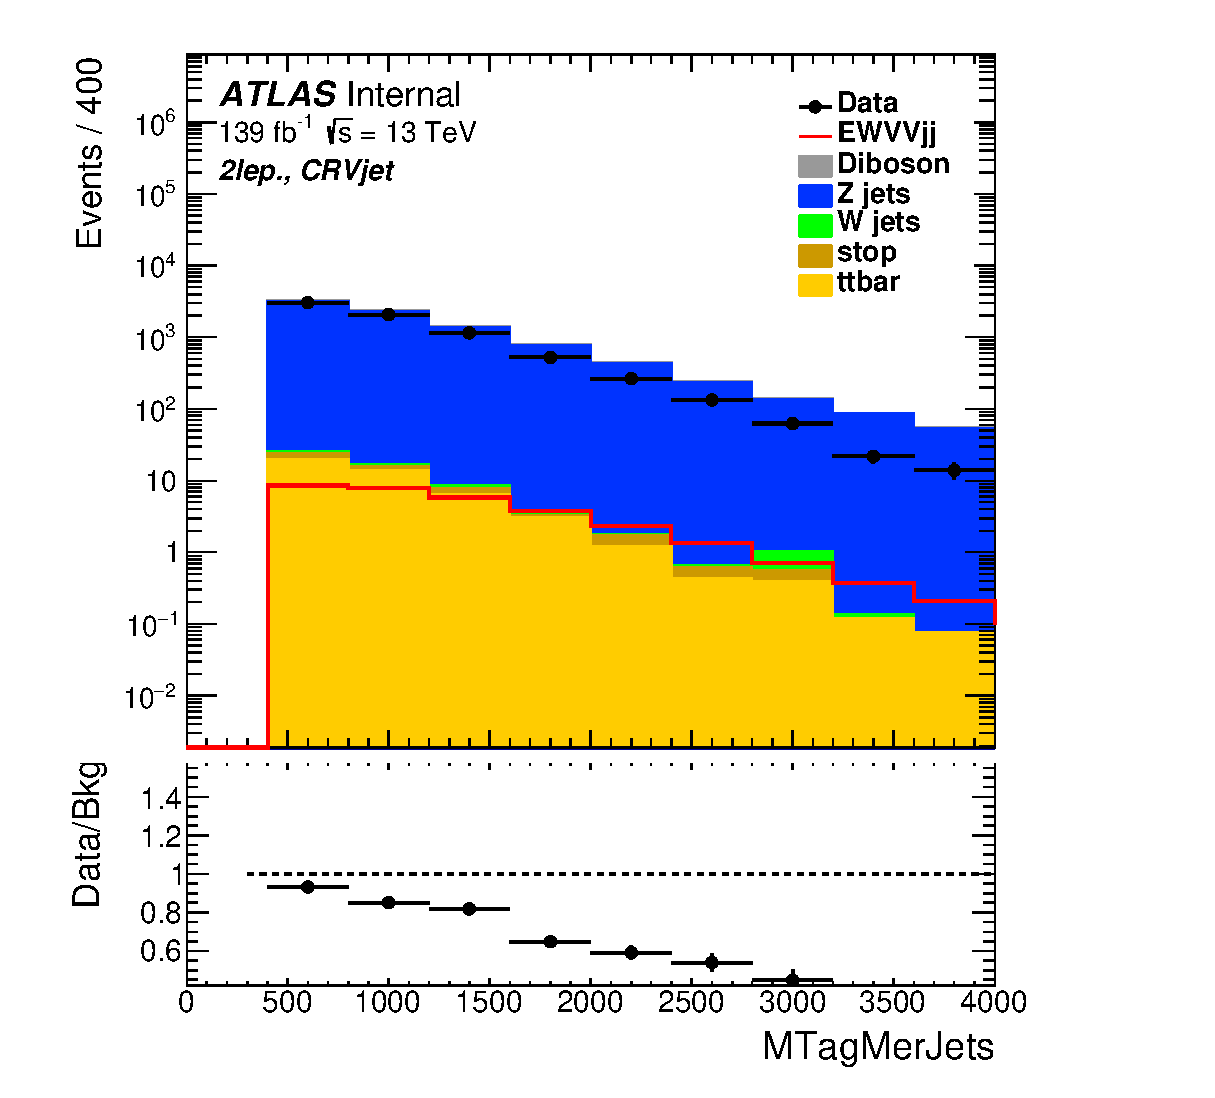
\includegraphics[width=0.45\textwidth]{figures/2lep/reweighting/before_reweighting/C_0ptag1pfat0pjet_0ptv_CRVjet_MTagMerJets_Log.eps}}
    \subfigure[]{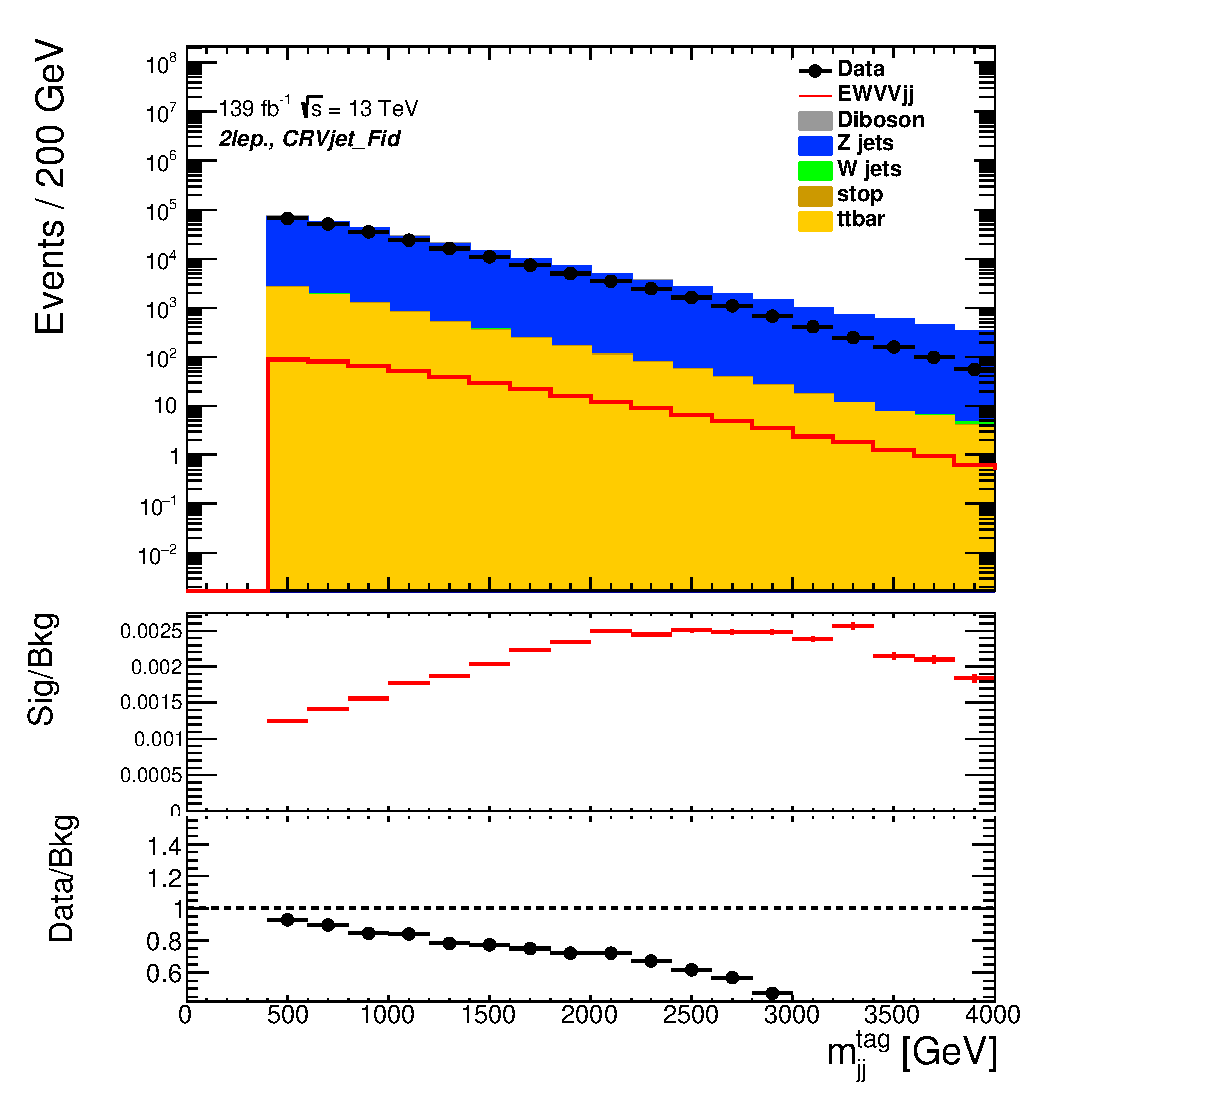
\includegraphics[width=0.45\textwidth]{figures/2lep/reweighting/before_reweighting/C_0ptag2pjet_0ptv_CRVjet_Fid_MTagResJets_Log.eps}}
    \caption{ $m^{tag}_{jj}$ distributions before applying reweighting for the merged (a) and resolved (b) control regions in the 2-lepton channel.}
    \label{fig:2lep_mtag_before_rw}
\end{figure}

The $Z$+jets production is the leading background for the 2-lepton analysis and contributes significantly for the 0-lepton analysis. The comparison of distributions from data and MC for various kinematic variables after re-weighting in the 2-lepton Z+jets merged and resolved control region are shown in Figure \ref{fig:2lep_zjets_merged_CR} and Figure \ref{fig:2lep_zjets_resolved_CR}
respectively. 


% 2-lepton new merged CR - plots
%\begin{figure}[ht]
%    \centering
%    \subfigure[]{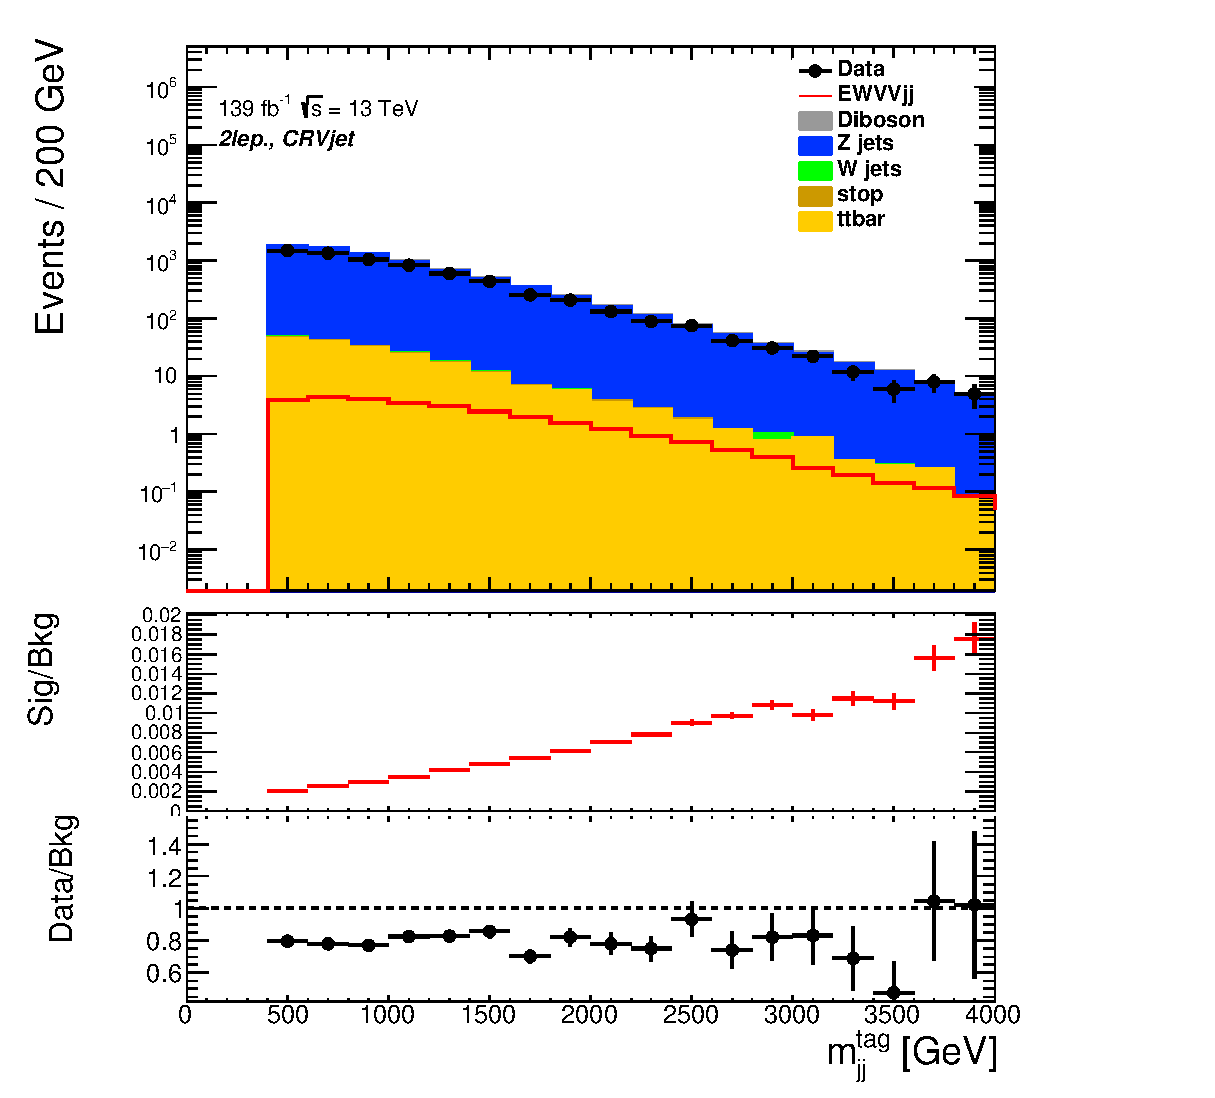
\includegraphics[width=0.45\textwidth]{figures/2lep/reweighting/after_reweighting/C_0ptag1pfat0pjet_0ptv_CRVjet_MTagMerJets_Log.eps}}
%    \subfigure[]{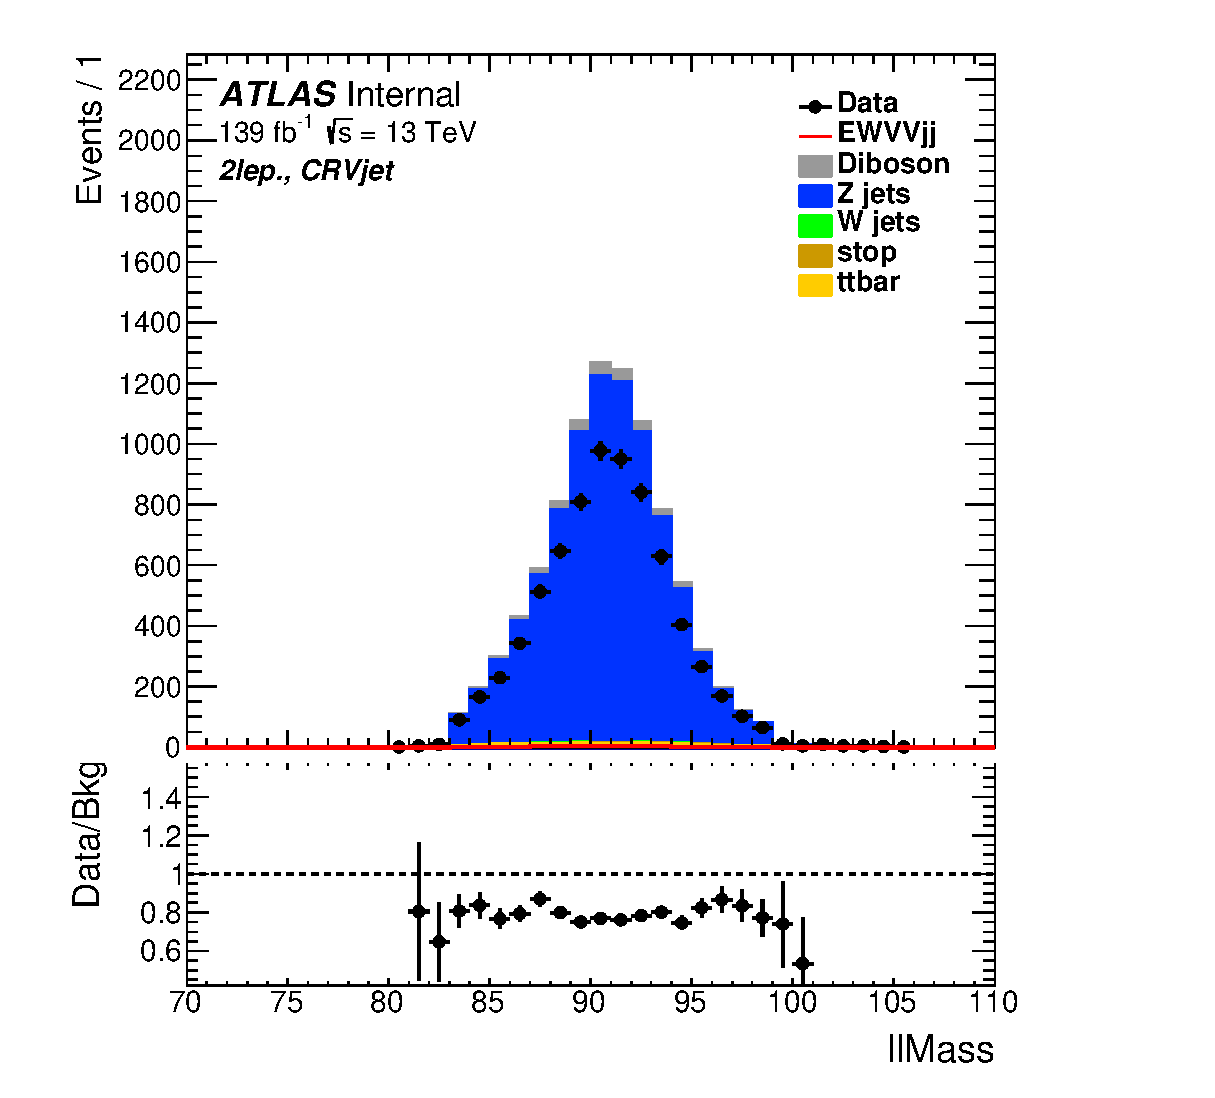
\includegraphics[width=0.45\textwidth]{figures/2lep/reweighting/after_reweighting/C_0ptag1pfat0pjet_0ptv_CRVjet_llMass_Lin.eps}}
%    \subfigure[]{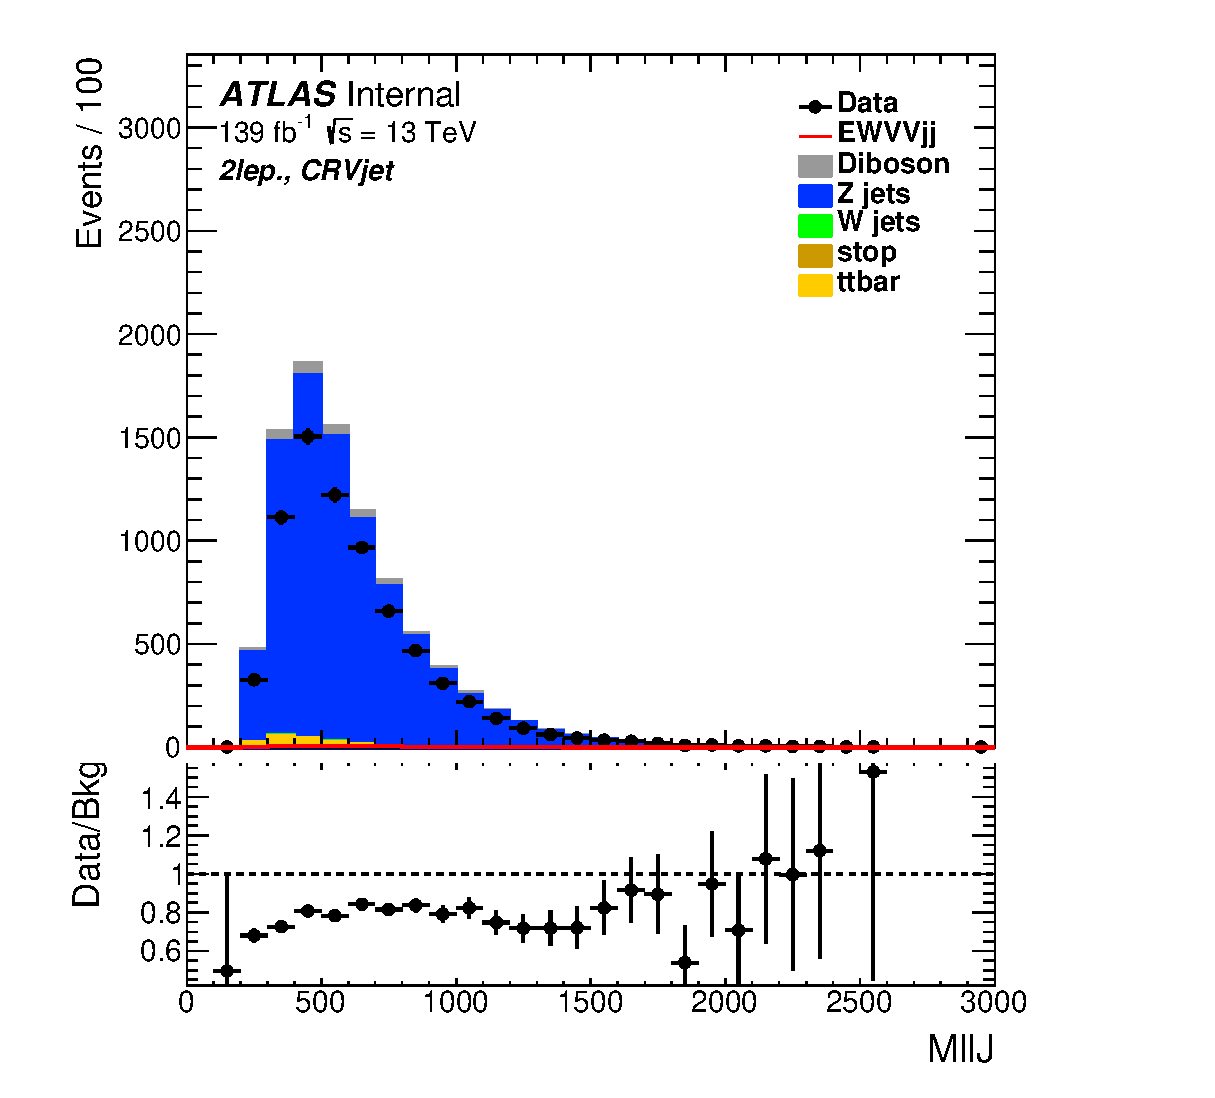
\includegraphics[width=0.45\textwidth]{figures/2lep/reweighting/after_reweighting/C_0ptag1pfat0pjet_0ptv_CRVjet_MllJ_Lin.eps}}
%    \subfigure[]{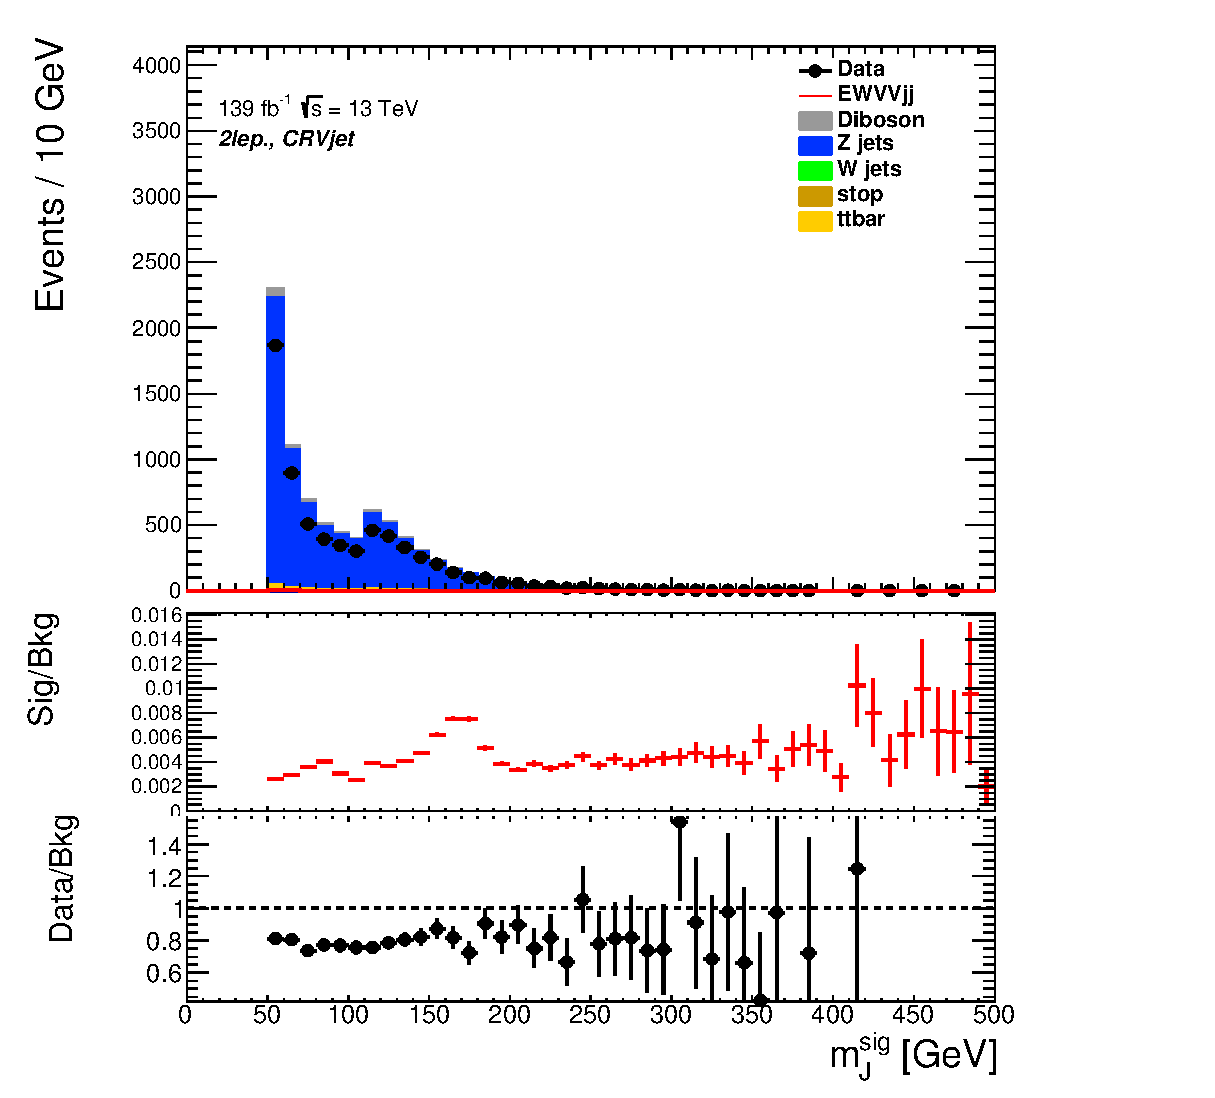
\includegraphics[width=0.45\textwidth]{figures/2lep/reweighting/after_reweighting/C_0ptag1pfat0pjet_0ptv_CRVjet_fatJetMass_Lin.eps}}
%    \caption{ Various kinematic variables in the Z+jets merged CR in the 2-lepton channel analysis.}
%    \label{fig:2lep_zjets_merged_CR}
%\end{figure}


% 2-lepton resolved CR fiducial- plots
%\begin{figure}[ht]
%    \centering
%    \subfigure[]{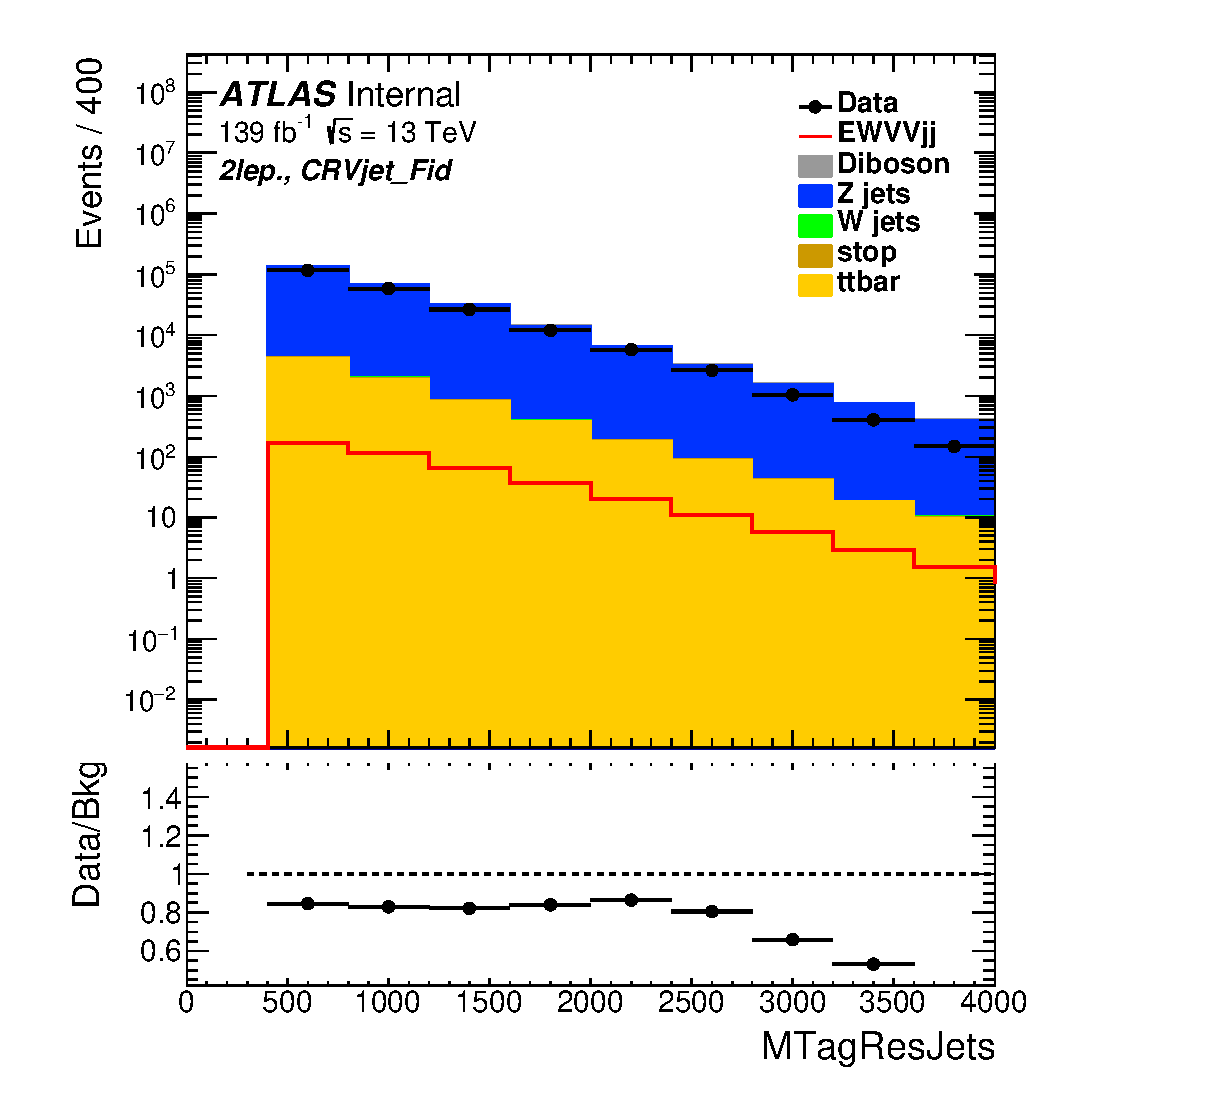
\includegraphics[width=0.45\textwidth]{figures/2lep/reweighting/after_reweighting/C_0ptag2pjet_0ptv_CRVjet_Fid_MTagResJets_Log.eps}}
%    \subfigure[]{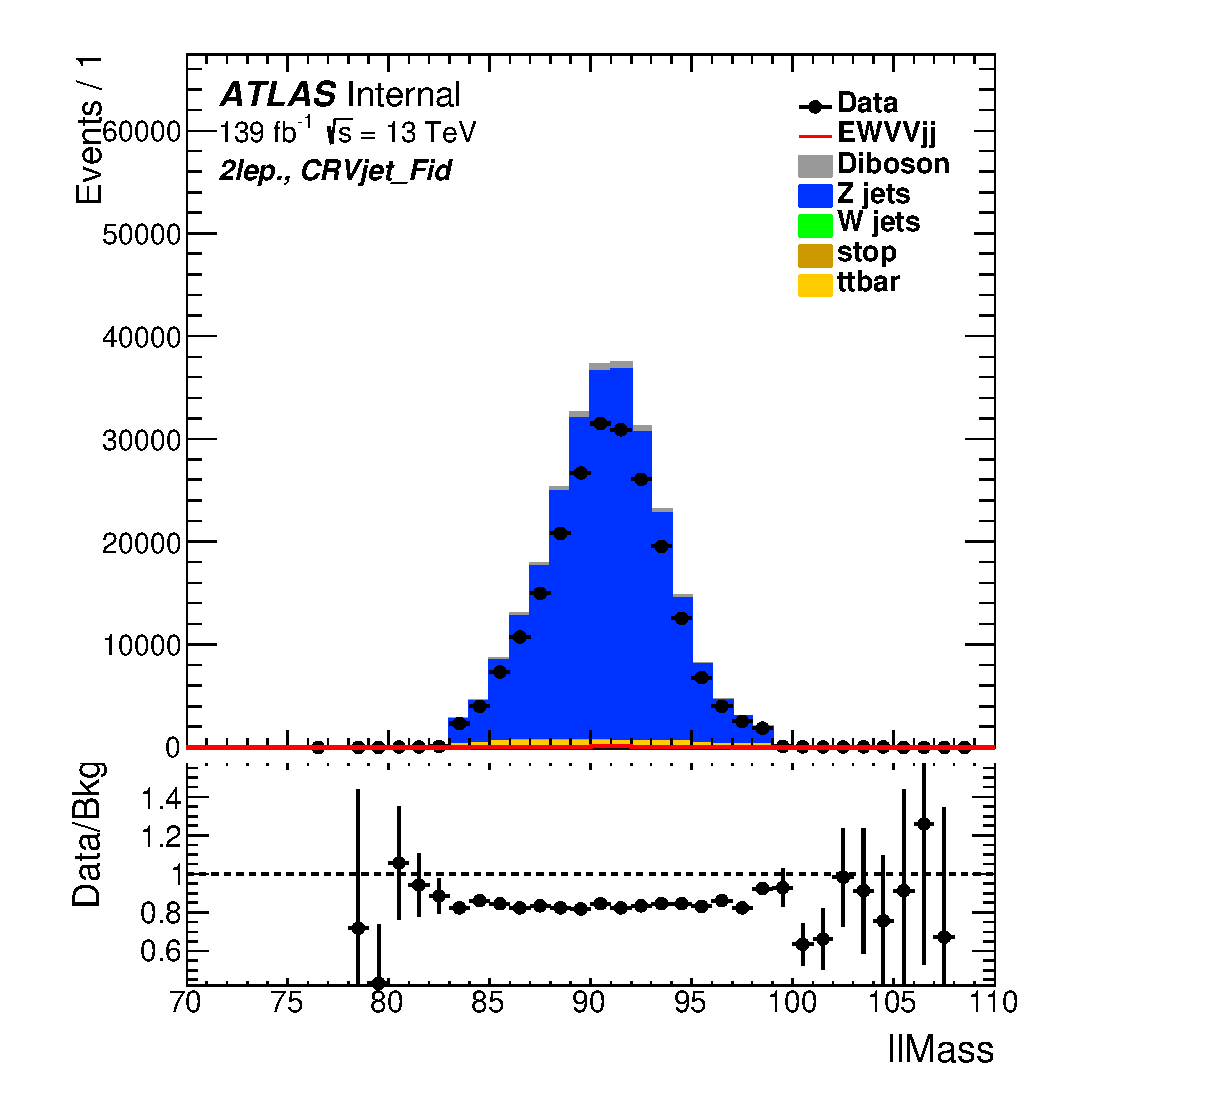
\includegraphics[width=0.45\textwidth]{figures/2lep/reweighting/after_reweighting/C_0ptag2pjet_0ptv_CRVjet_Fid_llMass_Lin.eps}}
%    \subfigure[]{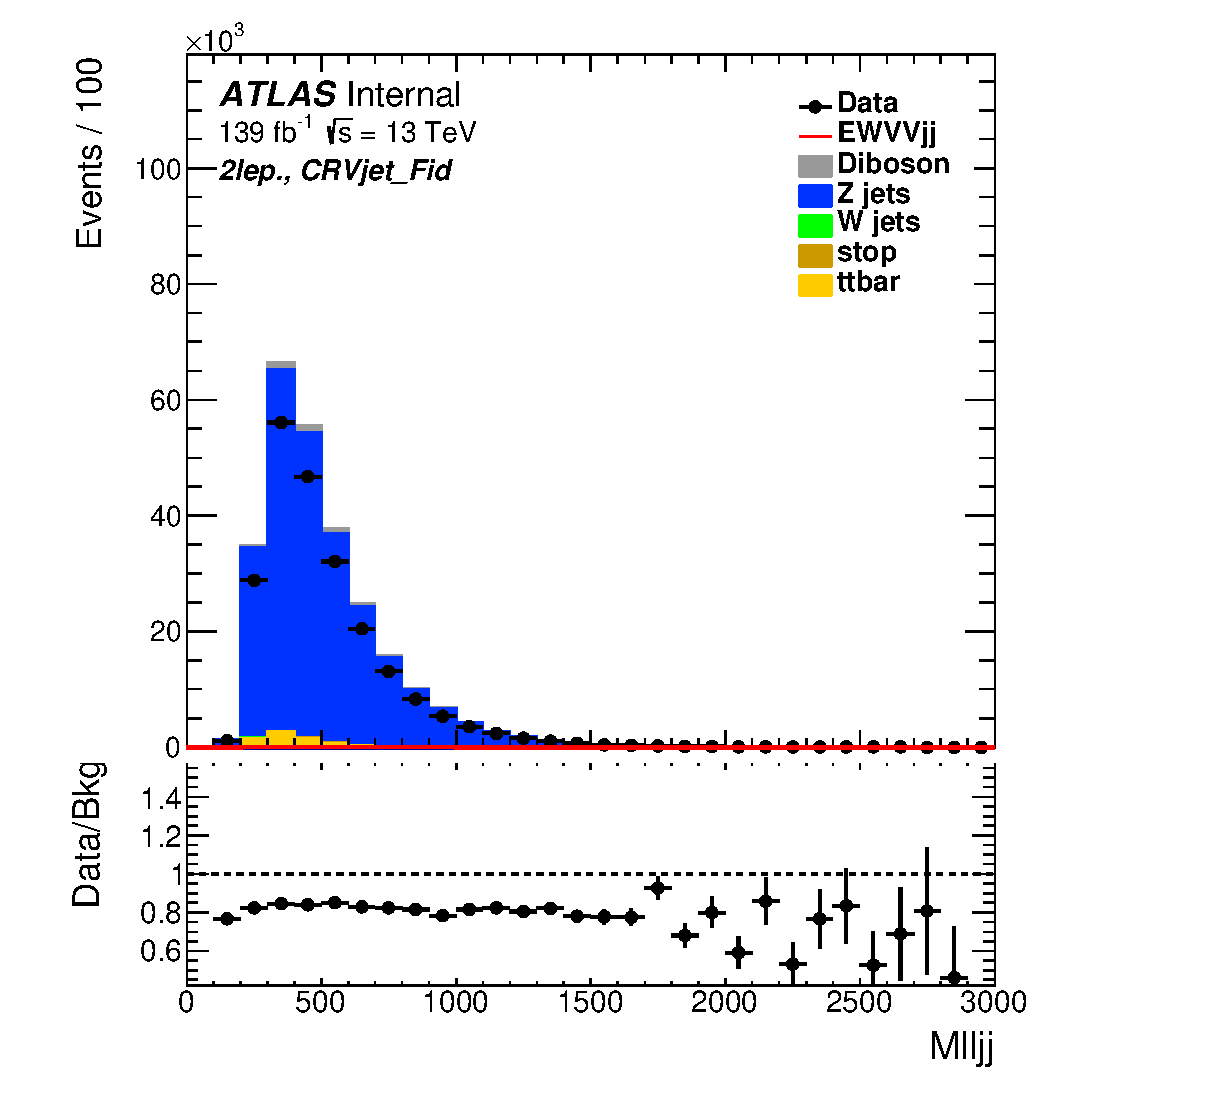
\includegraphics[width=0.45\textwidth]{figures/2lep/reweighting/after_reweighting/C_0ptag2pjet_0ptv_CRVjet_Fid_Mlljj_Lin.eps}}
%    \subfigure[]{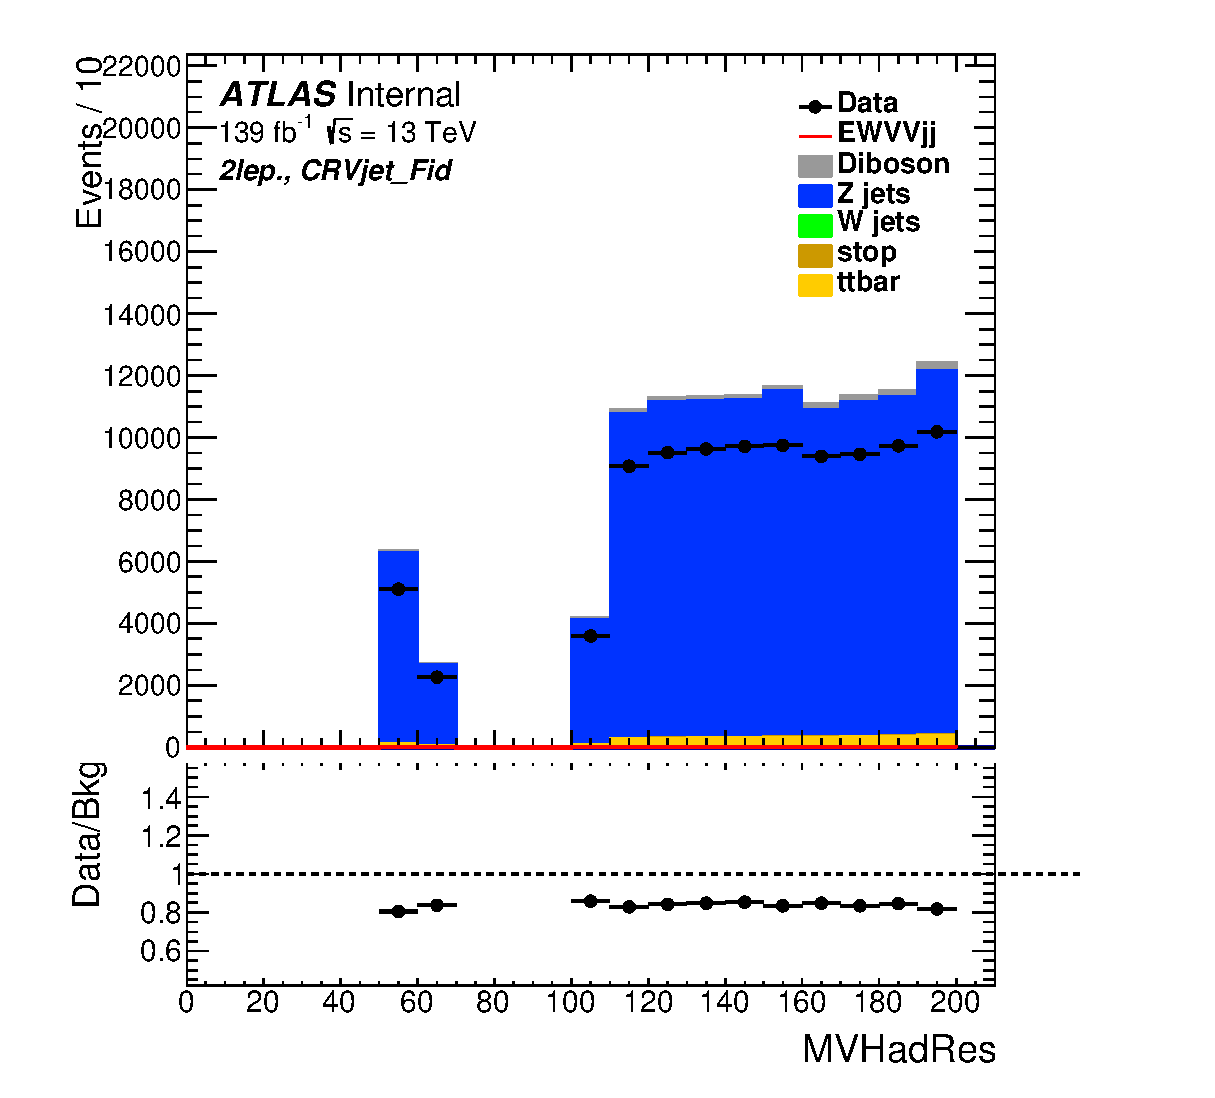
\includegraphics[width=0.45\textwidth]{figures/2lep/reweighting/after_reweighting/C_0ptag2pjet_0ptv_CRVjet_Fid_MVHadRes_Lin.eps}}
%    \subfigure[]{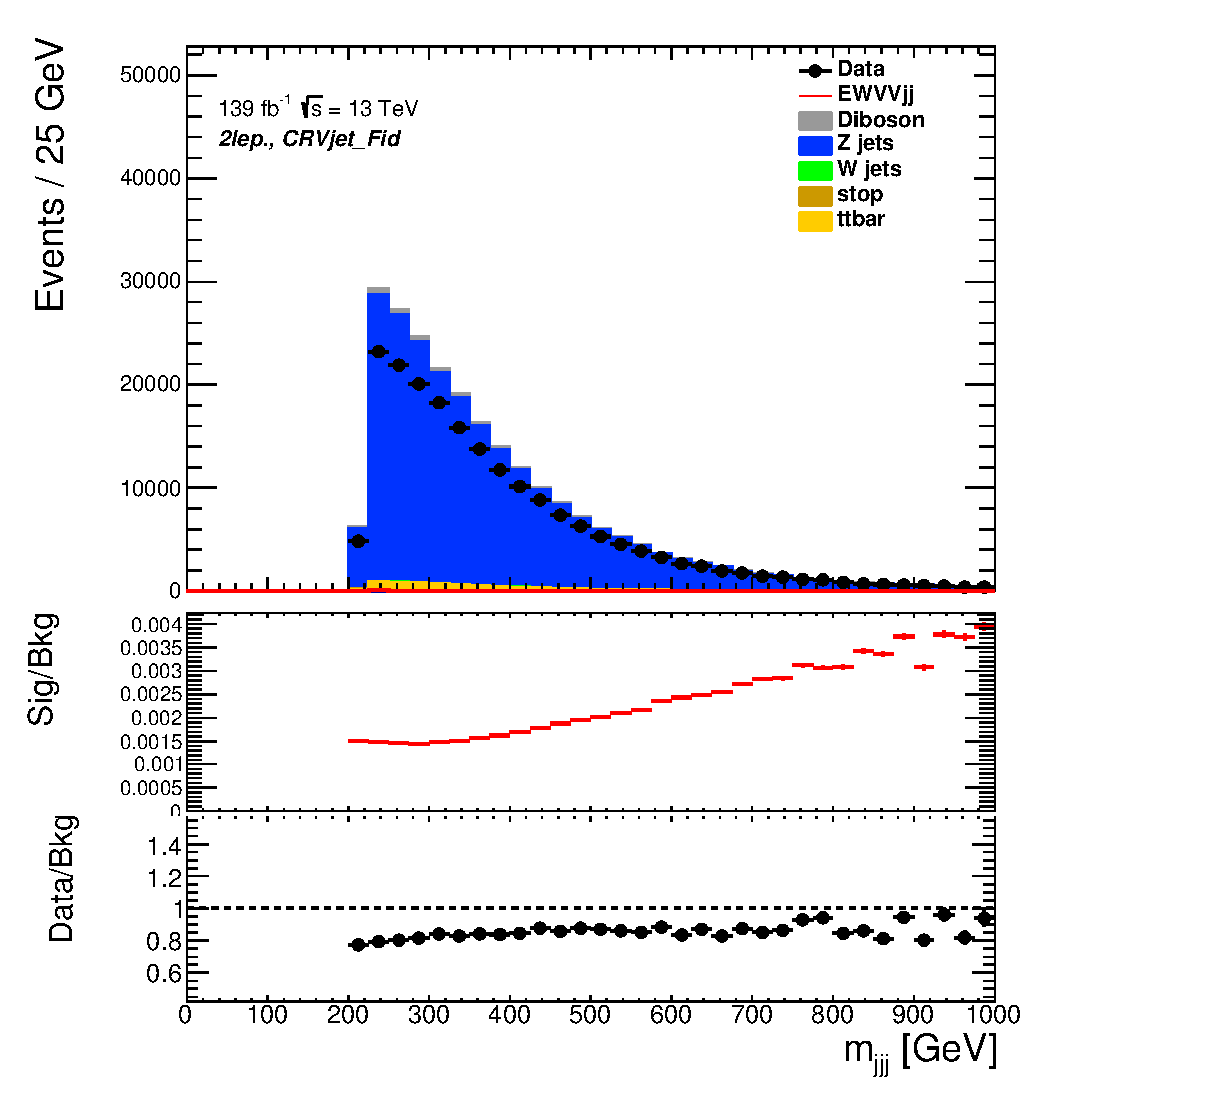
\includegraphics[width=0.45\textwidth]{figures/2lep/reweighting/after_reweighting/C_0ptag2pjet_0ptv_CRVjet_Fid_topMass_Lin.eps}}
 %   \caption{ Various kinematic variables in the Z+jets resolved CR in the 2-lepton channel analysis.}
  %  \label{fig:2lep_zjets_resolved_CR}
%\end{figure}

